\documentclass[12pt,pdf,hyperref={unicode}]{beamer}
%\usetheme{boxes}
\beamertemplatenavigationsymbolsempty
\setbeamertemplate{footline}[page number]
% Set it for the internal PhD thesis defence to reduce number of slides
%\setbeamersize{text margin left=0.5em, text margin right=0.5em}

\usepackage[utf8]{inputenc}
%\usepackage[english, russian]{babel}
\usepackage{bm}
\usepackage{multirow}
\usepackage{ragged2e}
\usepackage{indentfirst}
\usepackage{multicol}
\usepackage{subfig}
\usepackage{amsmath,amssymb}
\usepackage{enumerate}
\usepackage{mathtools}
\usepackage{comment}
\usepackage[all]{xy}
\usepackage{tikz}
\usetikzlibrary{positioning,arrows}
\tikzstyle{name} = [parameters]
\definecolor{name}{rgb}{0.5,0.5,0.5}

%\usepackage{caption}
%\captionsetup{skip=0pt,belowskip=0pt}

%\newtheorem{theorem}{Theorem}
%\newtheorem{statement}{Statement}
%\newtheorem{definition}{Definition}

% colors
\definecolor{darkgreen}{rgb}{0.0, 0.2, 0.13}
\definecolor{darkcyan}{rgb}{0.0, 0.55, 0.55}
%\AtBeginEnvironment{figure}{\setcounter{subfigure}{0}}
%\captionsetup[subfloat]{labelformat=empty}

%----------------------------------------------------------------------------------------------------------

\title{ Put the title of your thesis \\ here}
%\author{Name Surname}
%\institute[]{}
%\date{2024}

%---------------------------------------------------------------------------------------------------------
\begin{document}
%\begin{frame}
%\titlepage
%\end{frame}
\setcounter{page}{2}%remove here for the title
%----------------------------------------------------------------------------------------------------------
%\section{Please do not use sectioning in the presentations}
\begin{frame}{StyleDomain: Efficient and Lightweight Parameterizations of StyleGAN}
Generative AI is one of the latest famous technologies. It uses for image generation, style transfer, video generation and etc.
\begin{block}{The problem}
How to adapt GAN model to a specific domain with few samples (paintings by artists, pop art, graffiti)?
\end{block}
\begin{block}{The method}
Affine+ and AffineLight parametrization method
\end{block}
\begin{block}{The solution} 
\begin{enumerate}[1)]
\item Combination several affine layers and one convolutional block from the synthesis network on domain adaptation
\item Affine and Affine+ parametrization methods is efficient for dissimilar domains
\end{enumerate}
\end{block}
\end{frame}
%----------------------------------------------------------------------------------------------------------
\begin{frame}{Affine parametrization result}
Example applies of five parametrization methods for domains: cat and dog.
\begin{columns}
\begin{column}{0.3\textwidth}
Fid (Fréchet inception distance) metric use to defined model quality.
\end{column}
\begin{column}{0.7\textwidth}
	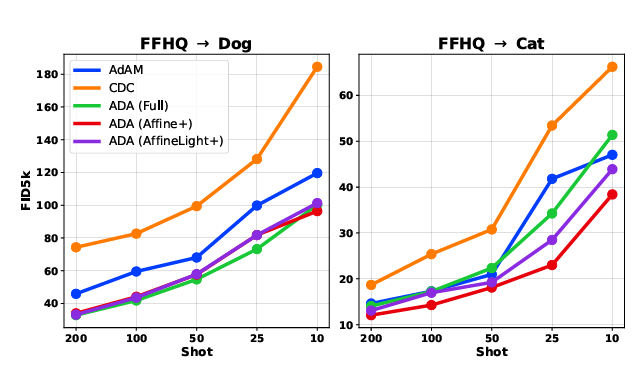
\includegraphics[width=1\textwidth]{ffhq_dataset_example_training}      
\end{column}
\end{columns}
\bigskip
Parametrization family Affine shows the better results than others
\end{frame}
\end{document}